
%(BEGIN_QUESTION)
% Copyright 2013, Tony R. Kuphaldt, released under the Creative Commons Attribution License (v 1.0)
% This means you may do almost anything with this work of mine, so long as you give me proper credit

A 200 newton weight is suspended by a hinged strut, which is kept at an angle of 30$^{o}$ by the tension in a cable.  Determine the compressive force within the strut as well as the tension within the cable.  Assume that the cable is perfectly horizontal and that the strut is weightless:

$$\includegraphics[width=15.5cm]{i02647x01.eps}$$

$F_{strut}$ = \underbar{\hskip 50pt} N

\vskip 10pt

$F_{cable}$ = \underbar{\hskip 50pt} N

\vskip 10pt

\underbar{file i02647}
%(END_QUESTION)





%(BEGIN_ANSWER)

$F_{strut}$ = {\bf 400 N}

\vskip 10pt

$F_{cable}$ = {\bf 346.4 N}

%(END_ANSWER)





%(BEGIN_NOTES)


%INDEX% Mathematics review: trigonometric calculations

%(END_NOTES)


